\def\pathToRoot{.}
\documentclass[a4paper, 12pt]{article}

\usepackage[utf8]{inputenc}
\usepackage{ifthen}
\usepackage{xparse}
\usepackage{scrextend}
\usepackage{setspace}
\usepackage{verbatim}
\usepackage{color}
\usepackage[inline]{enumitem}
\usepackage[colorlinks=true, linkcolor=black, citecolor=black]{hyperref}

\usepackage{tikz}
\usepackage{pgfplots}
\usepackage{bbold}
\usepackage{listings}

\usepackage{subcaption}

\usepackage{amsmath}
\usepackage{amssymb}
\usepackage{latexsym}
\usepackage{hyperref}
\usepackage{cleveref}

\definecolor{gray}{rgb}{0.2,0.2,0.2}

\pagenumbering{arabic}


\usepackage[a4paper, left=2cm, top=2cm, right=2cm, bottom=2cm]{geometry}

\usepackage{multirow}
\usepackage{fancyvrb}

\newcommand{\vect}[1]{\boldsymbol{#1}}

\newcounter{exerciseCounter}
\setcounter{exerciseCounter}{0}

\newcommand{\exerciseNumber}{\sheetnumber.\arabic{exerciseCounter}}

\setenumerate{label=\alph*)}

% Sheet Header
\newcommand{\exercisehead}[3]
{
    \def\sheetnumber{#1}
    \begin{center}
        \begin{minipage}{0.45\linewidth}
            \textsc{Universität des Saarlandes}
            \par
           Prof. Dr. Dietrich  Klakow
           \par
           Lehrstuhl für Signalverarbeitung
           \par
           NNIA Winter Term 2019/2020
        \end{minipage}
        \begin{minipage}{0.45\linewidth}
            \begin{flushright}
               
\includegraphics[width=0.30\linewidth]{headers/lsv_logo.jpg}
            \end{flushright}
        \end{minipage}
        \vspace{5pt}
        \hrule
        \vspace{12pt}
        \doublespacing
        {
            \LARGE
            \textbf{Exercise Sheet #1}
        }
        \par
        {
            \large
            #2
        }
        \par
        \ifdefined\issolution
        \textit{(Solutions)}
        \else
        \fi
        
    \textbf{Deadline: #3}

    \end{center}
    \vspace{2pt}
    \hrule
    \vspace{12pt}
}

% Exercise environment
\NewDocumentEnvironment{exercise}{oo}
{
	\refstepcounter{exerciseCounter}
	\par
	\vspace{12pt}
    \noindent
    \textbf{Exercise \exerciseNumber \  - #1}\IfNoValueF{#2}{\hfill(#2 points)}
	\vspace{12pt}
	\par
	\begin{addmargin}[12pt]{0pt}
}
{
    
	\end{addmargin}
	\par
	\vspace{12pt}
}

% Solution environment
\newenvironment{solution}
{
		\ifthenelse{\isundefined{\issolution}}
		{
			\comment
		}
		{
			\par
			\color{gray}
			\vspace{6pt}
			\textit{Solution \exerciseNumber}
			\par
			\begin{addmargin}[30pt]{0pt}
		}
}
{
		\ifthenelse{\isundefined{\issolution}}
		{
		}
		{
			\end{addmargin}
			\par
			\vspace{12pt}
		}
}



\def\issolution{}

\begin{document}

% {Sheet number}{headline}{deadline}
\exercisehead{7}{\small Philip Georgis [s8phgeor], Pauline Sander [s8pasand], Vilém Zouhar [vizo00001] }{12. 1. 2021}

\section*{Exercises}

\newcommand{\TODO}[1]{\textcolor{red}{TODO:#1}}

\begin{exercise}[Norm Penalty]

\begin{enumerate}
    \item Assuming the output of the layer is some distribution, biases shift the distribution, but do not change its shape (they only influence one variable). It is also easier to approximate the bias better (less data is needed), simply by shifting the distribution to true distribution mean. We need to regularize the weights, because they model the interaction between variables, which can pick up noise from the training data, increase training and decrease test performance (overfitting). Biases, on the other hand, are less prone to overfitting. Regularizing them could lead to underfitting.
    \item The \textit{Class} coefficient would be penalized more, because without regularization it is much higher ($17.28$) than for the \textit{Age} variable ($0.03$). The new loss function would be a sum of upward facing parabolas. This is the reason why input variables are sometimes z-normed. The larger variable would be penalized more in an absolute value, but less proportionally to the original value, because it is more important. This can be demonstrated with the original code. The new coefficients are: $0.03$ and $-17.24$, which are $97\%$ and $99\%$ of the original values.
% Code for this claim.
%     model = Ridge(alpha=1).fit(titanic[['Age', 'Pclass']], titanic['Price'])
% print(f'CoefA: {model.coef_[0]:.4f}, CoefPC: {model.coef_[1]:.4f}, Offset: {model.intercept_:.2f}')
% model = LinearRegression().fit(titanic[['Age', 'Pclass']], titanic['Price'])
% print(f'CoefA: {model.coef_[0]:.4f}, CoefPC: {model.coef_[1]:.4f}, Offset: {model.intercept_:.2f}')
    \item $L^1$ regularization can lead to results with sparse parameters. This can be seen in Fig. \ref{fig:my_label}, where the $L^1$ norm leads to $w_1$ being 0. Since their parameters are zero, we can remove the more irrelevant features altogether. We select the more `important' features. 
    \begin{figure}[h!]
        \centering
        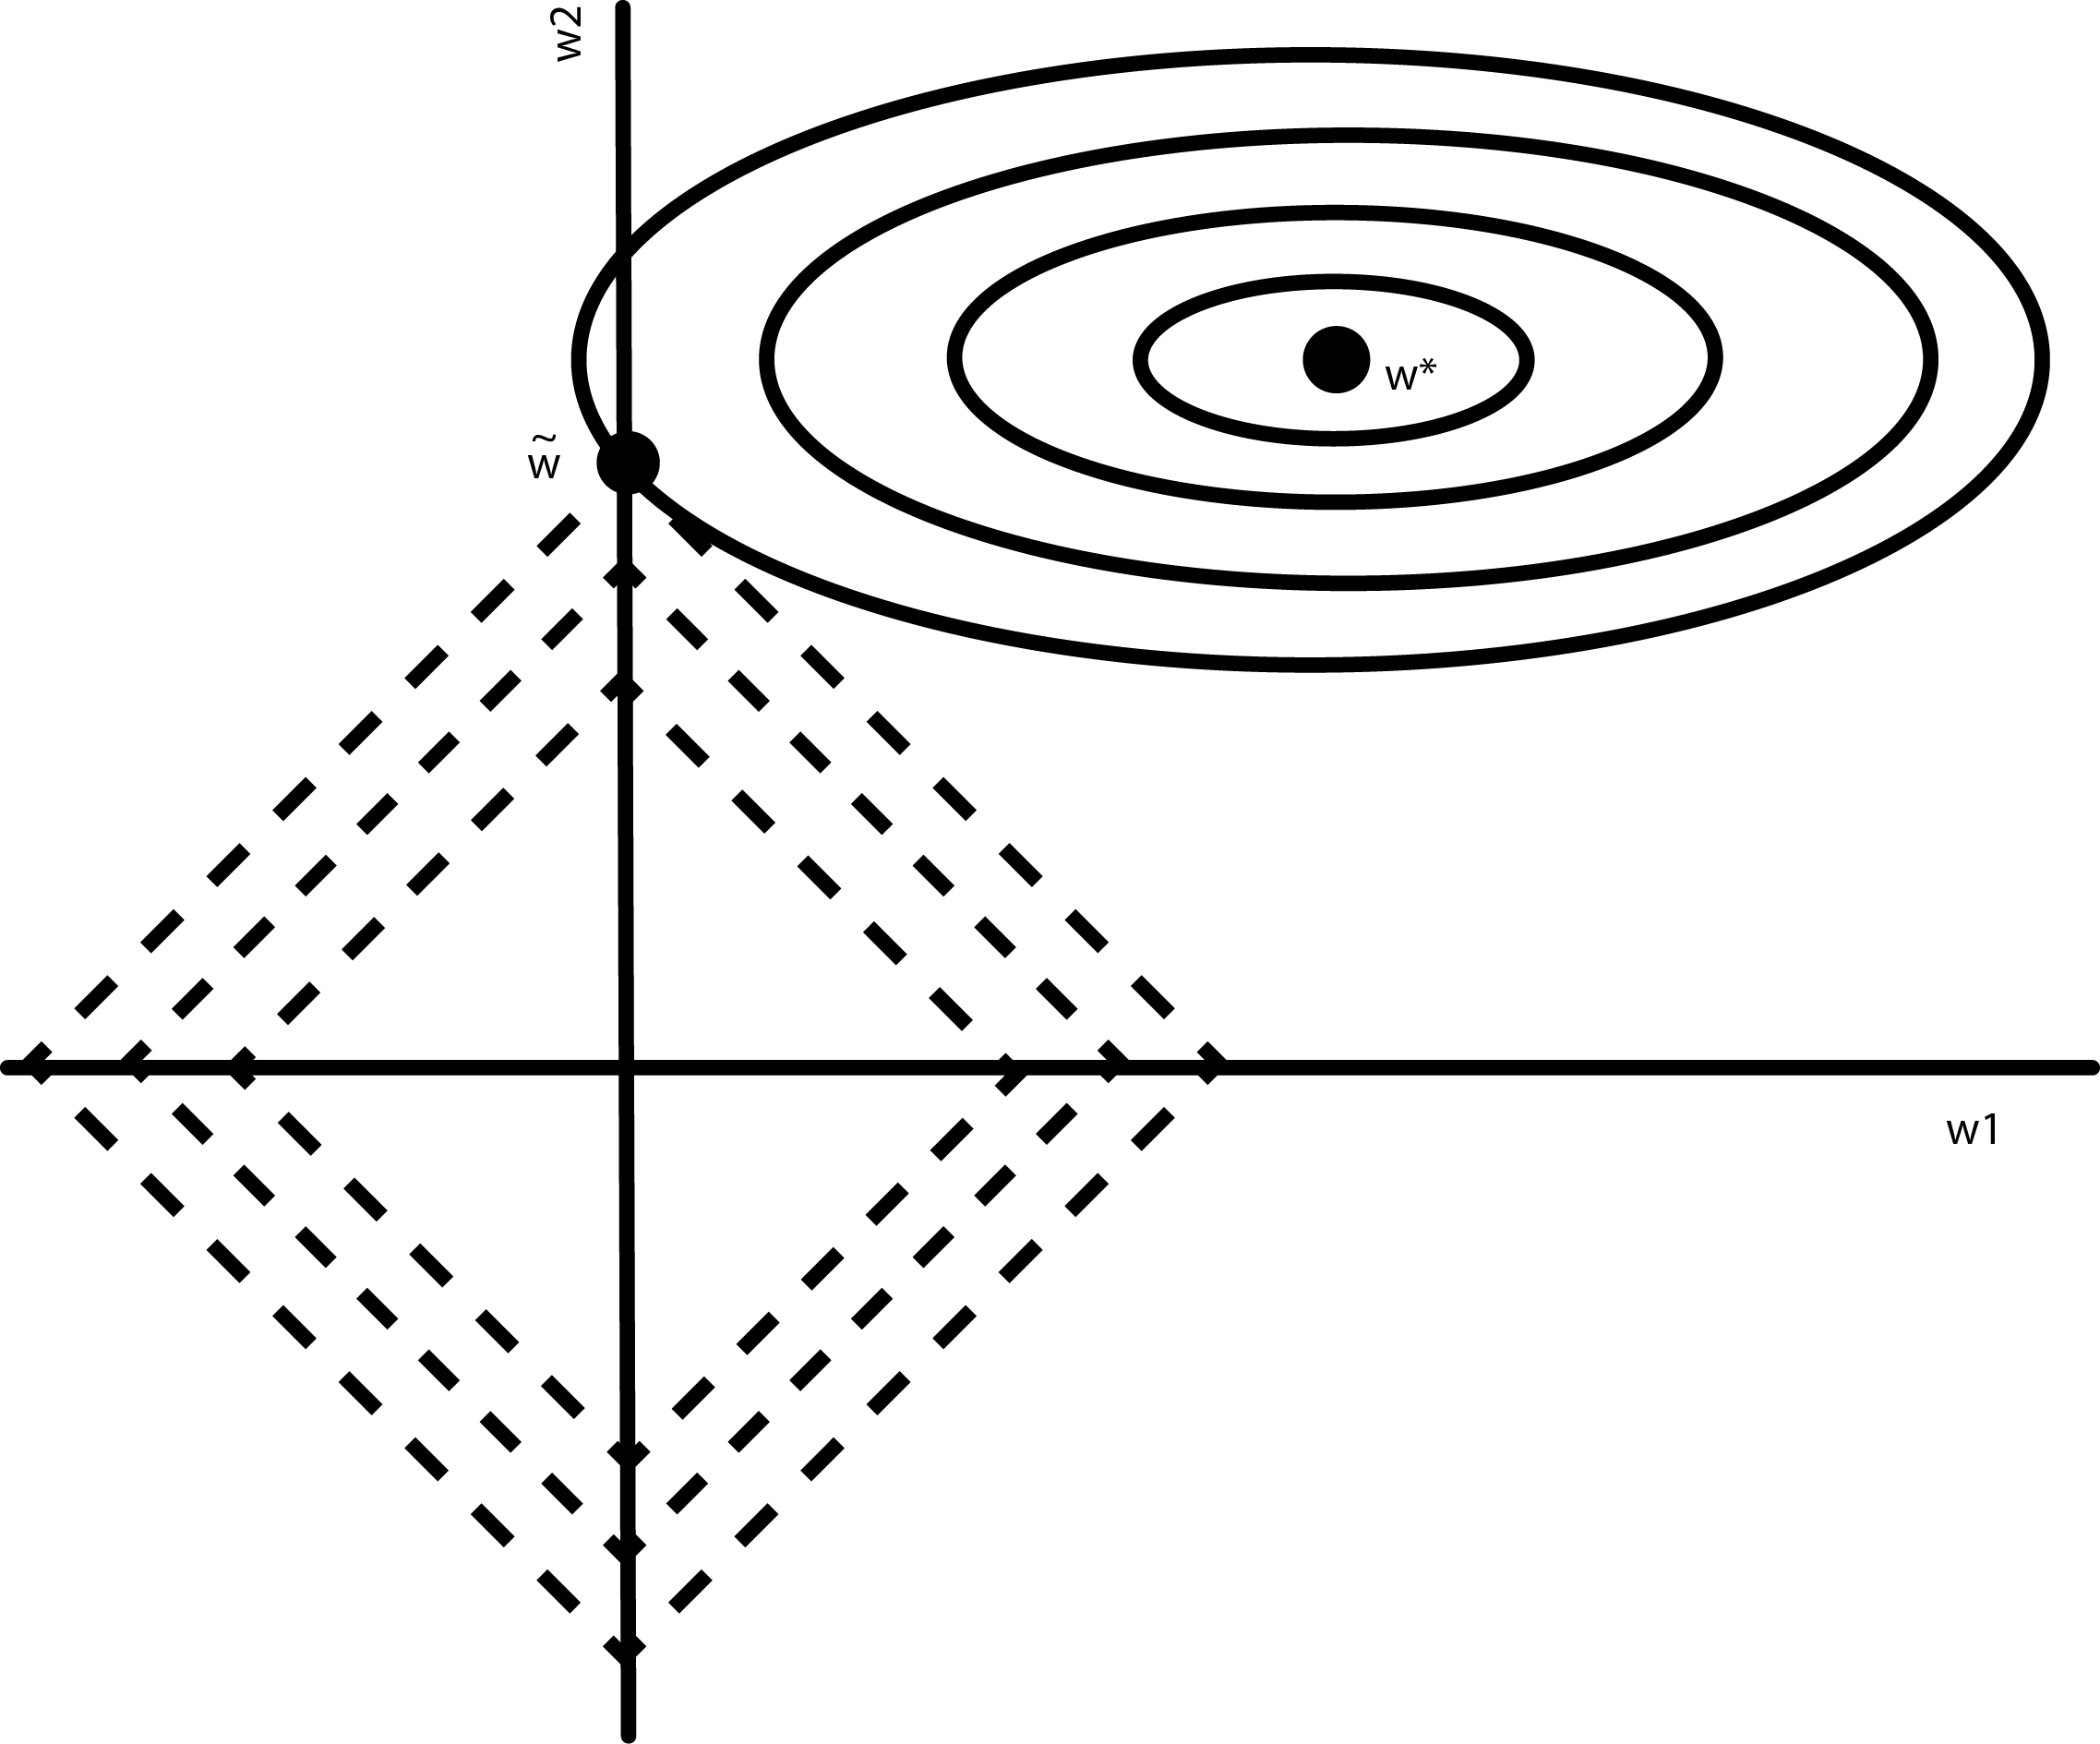
\includegraphics[scale=0.5]{img/L1_norm.png}
        \caption{$L^1$ regularization}
        \label{fig:my_label}
    \end{figure}
\end{enumerate}
\end{exercise}

\begin{exercise}[Dataset Augmentation]

\begin{enumerate}
    \item For vision tasks, it is relatively easy (methodically and computationally) to create augmented data with affine transformations or any other filter. The NLP data augmentation methods require more care, time and sometimes even whole pipeline. An example of this would be backtranslation. If this would be done on the go, then it would mean loading the reverse model into GPU, translating and decoding it and finally filtering by quality. It makes much more sense to do this beforehand with large batches.
    \item For machine translation and similar tasks, such as MT quality estiation, the backtranslation is a double-edged sword. Sometimes the corpus (e.g. ParaCrawl) may already be a product of publicly available MT systems. Translating it yet again leads to translationese, which hurts the language modelling capabilities of the model. On the other hand, model distillation has been shown to provide significant boosts, especially in early epochs of training. 
    \item If we perform it before splitting the data, we have to also keep the original data around, because they are used for evaluation and we want to evaluate on authentic data. Performing it after solves this issue, but we will end up augmenting the same example $k-1$ times.
    \item The size of the training set does not \textit{necessarily} determine the proportion of the data to be augmented. However, given that models are more prone to overfitting on smaller training sets, higher proportions of augmented data would certainly be beneficial in such situations by significantly increasing the amount of available training data. Larger datasets do also benefit from augmentation, though augmenting every item in a large dataset would not be as beneficial against overfitting as doing the same on a smaller dataset.
\end{enumerate}

\end{exercise}

\begin{exercise}[Bagging and Dropout]
\begin{enumerate}
    \item In dropout we obscure (randomly) some of the weights for a particular example, which can be seen as training multiple ensembled networks with unobscure weights shared. This is a bit similar to bagging, where each network is trained on sampled dataset in which case there is a probability that there are elements it will never encounter.
    \item No, because we want to make use of all of the features given to us. For vanilla dropout we need to multiply the whole layer by the probability so that the output distribution shape is the same.\\
    \linebreak
    \item
    \begin{lstlisting}
def inverse_dropout(layer, prob):
    # matrix of [0, 1]
    mask = rand(shape=layer.shape) < prob
    return ( layer @ mask ) / ( 1 - prob ) 
    \end{lstlisting}
\end{enumerate}
\end{exercise}

\begin{exercise}[Adversarial Training in NLP]
In computer vision, small amounts of noise added to images can result in erroneous outputs (e.g. misclassification or incorrect identification of images), despite being visually imperceptible to humans. In the NLP domain, even small perturbations are not completely imperceptible to humans. Methods for adversarial training in NLP, thus, parallel those of data augmentation in order for small changes not to disrupt the predictions of a model.
\begin{enumerate}
    \item \textbf{Synonym Replacement:} This technique substitutes individual words in a text with semantically related words. The result is a new training example with virtually unchanged meaning, simply using different words, which can increase the robustness of the model, e.g.:\\
    Original: \textit{This \textbf{film} displayed a \textbf{wealth} of inspiration on the part of the director.}\\
    Adversarial: \textit{This \textbf{movie} displayed an \textbf{abundance} of inspiration on the part of the director.}
    \item \textbf{Character Changes:} The effect of adding random noise to images can be modelled by intentionally misspelling words or changing individual characters in a text. This is performed in such a way that it models common misspellings or typos, so that it causes no comprehension problems for human readers, yet would trip up the model, e.g.:\\
    Original: \textit{Their \textbf{role} in the process should \textbf{definitely} not be discounted.}\\
    Adversarial: \textit{Their \textbf{roll} in the process should \textbf{definietly} not be discounted.}\\
    \item \textbf{Distractor Sentences:} Adversarial examples can also be generated by inserting distracting sentences, which would mislead a model but not a human reader. For example, given a text
    ``\textit{Following her studies in Athens, Maria was soon offered a job in Berlin. Maria moved to Berlin in 2007.}" and the question: ``\textit{Where did Maria move in 2007?}", an adversarial example can be constructed by adding to the original text a distractor sentence, which perturbs the sentence which contains the correct answer, e.g. ``\textit{Katerina moved to Thessaloniki in 2007.}". This could cause a QA model to answer ``Thessaloniki" rather than ``Berlin". \\
    \item \textbf{Syntactic Perturbations:} This technique creates adversarial training examples by perturbing the syntactic structure of sentences without changing their meaning. For example, hedges or fillers might be inserted, or constituents might be reordered to produce a semantically equivalent but distorted sentence, e.g.: \\
    Original: \textit{The best student in the class is eating lunch by himself.} \\
    Adversarial: \textit{You know, the student eating lunch by himself is perhaps the best in the class.}
    

\end{enumerate}
\textbf{Sources:}\\
https://nlpblog.cl.uni-heidelberg.de/index.php/2019/09/20/adversarial-training/
\\
https://towardsdatascience.com/what-are-adversarial-examples-in-nlp-f928c574478e
\\
https://nlp.stanford.edu/pubs/jia2017adversarial.pdf
\end{exercise}

\end{document}
